%!TEX root = ../gesamt.tex

\begin{Korollar}{
	Ist $f:[a,b] \rightarrow \mathbb{R}$ stetig, beziehungsweise monoton, beziehungsweise 
	besitzt $f$ höchstens endlich viele Unstetigkeitsstellen und ist beschränkt, so ist 
	$f \in \mathcal{R}_{[a,b]}$.
}\end{Korollar}

\begin{Bemerkung}{
	Mit Hilfe des Lebesguesches Integrabilitätskriterium kann man 
	sogar zeigen, dass beschränkte Funktionen mit abzählbar vielen Unstetigkeitsstellen 
	Riemann-integrierbar sind.
}\end{Bemerkung}

\begin{Beispiel}{
	\begin{align*}
		\int_0^a x \dd{x}
	\end{align*}
	Da $id :[0,a] \rightarrow \mathbb{R}$ stetig ist, existiert das Integral. \\
	Sei $P_n =\{ 0, \frac{a}{n}, \frac{2a}{n}, \hdots, \frac{(n-1)a}{n}, a\}$ 
	eine Partition von $[a,b]$. \\
	Es gilt: 
	\begin{align*}
		S(P_n, x) = & \sum_{i =1} ^n \frac{a_i}{n} \cdot \frac{a}{n} \\
		= & \frac{a^2}{n^2} \sum_{i = 1}^n i \\
		= & \frac{a^2}{n^2} \frac{n(n+1)}{2} \\ 
		= & \frac{a^2}{2} \cdot \left( 1 + \frac{1}{n} \right)
	\end{align*}
	\begin{align*}
		s(P_n, x) = & \sum_{i = 0}^n \frac{a_i}{n} \cdot \frac{a}{n}  \\
		= & \frac{a^2}{n^2} \cdot \frac{(n-1)n}{2} \\
		= & \frac{a^2}{2}\left( 1 - \frac{1}{n} \right)
	\end{align*}
	Da $id$ integrierbar ist, gilt:
	\begin{align*}
		\int_0^a x \dd{x} \in \left[ s(P_n,x), S(P_n, x)\right] = 
		\left[\frac{a^2}{2}- \frac{1}{n}, \frac{a^2}{2}+\frac{1}{n}\right]
		n \in \mathbb{N}
	\end{align*}
	Das heißt:
	\begin{align*}
		\int_0^a x \dd{x} \cap_{n \in \mathbb{N}} \left[\frac{a^2}{2}- \frac{1}{n}, 
		\frac{a^2}{2}+\frac{1}{n}\right]
	\end{align*}
	Also: $\int_0^a x \dd{x} = \frac{a^2}{2}$
}\end{Beispiel}

\begin{Beispiel}{
	Sei $D:[0,1] \rightarrow \mathbb{R}$ die \emph{Dirichlet-Funktion}, d.h
	\begin{align*}
		D(x) = \begin{cases}
			1 & \textit{falls } x \in \mathbb{Q} \\
			0 & sonst
		\end{cases}
	\end{align*}
	Daher gilt für jede Partition $P = \{x_0, \hdots, x_n\}$, dass 
	\begin{align*}
		M_i = & \sup_{x \in [x_{i-1}-x_i]} f(x) = 1 \text{ und}\\
		m_i = & \inf_{x \in [x_{i-1}-x_i]} f(x) = 0
	\end{align*}
	Damit gilt:
	\begin{align*}
		S(P,f) - s(P,f) = \sum_{i = 1}^n (M_i - m_i) \cdot \Delta x_i 
		= \sum_{i = 1}^n \Delta x_i = 1
	\end{align*}
	Ergo: $D$ ist nicht Riemann-integrierbar
}\end{Beispiel}

\begin{Satz}{\label{vl_11_satz23}
	Sei $f \in \mathcal{R}_{[a,b]}$ und $m \leq f(x) \leq M$ $ (x \in [a,b])$.\\
	Sei ferner $\Phi : [m, M] \rightarrow \mathbb{R}$ stetig. 
	Dann ist $\Phi \circ f \in \mathcal{R}_{[a,b]}$.
}\end{Satz}

\begin{proof}	
	 Sei $\epsilon > 0$ gegeben. Da $\Phi$ auf dem abgeschlossenen Intervall 
	$[m,M]$ stetig ist, existiert ein $\delta > 0$ 
	(Ohne Einschränkung sei $\delta < \epsilon$) mit :
	\begin{align*}
		\vert s - t\vert < \delta \Rightarrow \vert f(x) - f(t) \vert < \epsilon
	\end{align*}
	Da $f$ integrierbar ist, gibt es eine Partition $P = \{x_0, \hdots, x_n\}$
	mit 
	\begin{align*}
		S(P,f) - s(P,f) < \delta^2
	\end{align*}		
	Wie üblich bezeichnen wir 
	\begin{align*}
		M_i = & \sup_{x \in [x_{i-1}-x_i]} f(x) \text{ und } \\
		m_i = & \inf_{x \in [x_{i-1}-x_i]} f(x) \text{ und weiterhin} \\
		M_i^+ = & \sup_{x \in [x_{i-1}-x_i]} \Phi \circ f \text{ sowie } \\
		m_i^* = & \inf_{x \in [x_{i-1}-x_i]} \Phi \circ f(x)
	\end{align*}		
	Seien
	\begin{align*}
		A = & \{i = 1, \hdots, n \vert M_i -m < \delta \} \\
		B = & \{ i = 1, \hdots, n\} \setminus A
	\end{align*}
	Aufgrund der Wahl von $\delta$ gilt für alle $ i \in A: M_I^+ - m_i^* < \epsilon$
	Weiter gilt: 
	\begin{align*}
		\delta \cdot \sum_{i \in B} \Delta x_i = \sum_{i \in B} \delta \cdot \Delta x_i 
		\leq  \sum_{i \in B} (M_i - m_i) \Delta x_i \leq \delta^2
	\end{align*}
	Ergo: $\sum_{i \in B} \Delta x_i \leq \delta$. \\
	Damit gilt:
	\begin{align*}
		S(P, \Phi \circ f) - s(P, \Phi \circ f) = 
		& \sum_{i = 1}^n (M_i^+ - m_i^*) \cdot\Delta x_i  \\
		= & \sum_{i \in A} (M_i^+ - m_i^* ) \cdot \Delta x_i + 
			\sum_{i \in B} (M_i^+ -m_i) \Delta x_i \\
		\leq & \epsilon \sum_{i \in A}\Delta x_i + 2 \sup_{x \in [m,M]} \abs{
			\Phi \circ f} \cdot \sum_{i \in B} \Delta x_i \\
		\leq & \epsilon \left(|b-a| + 2\sup_{x \in [m,M]} \abs{\Phi \circ f(x)}\right)
	\end{align*}
	Da $\epsilon > 0$ beliebig, folgt die Behauptung mit~\ref{kap_10_satz18}.
\end{proof}

\begin{Satz}{\label{vl_11_satz24}%12
	Seien $f_1, f_2,f \in \mathcal{R}_{[a,b]}$ Dann gilt:
	\begin{enumerate}
		\item 
		\begin{align*}
			\int_a^b f_1 +f_2 \dd{x} = \int_a^b f_1\dd{x} + \int_a^b f_2 \dd{x}
		\end{align*}
		und für $c \in \mathbb{R}$ gilt:
		\begin{align*}
			\int_a^b c f\dd{x} = c \int_a^b f\dd{x}
		\end{align*}
		\item Insbesondere gilt also 
		\begin{align*}
			f_1 + f_2 \in \mathcal{R}_{[a,b]} \text{ und} \\
			c f \in \mathcal{R}_{[a,b]}
		\end{align*}
		\item Gilt $f_1(x) \leq f_2(x) \text{ } ( x \in [a,b])$ so folgt
		\begin{align*}			
			\int_a^b f_1 \dd{x} \leq \int_a^b f_2 \dd{x}
		\end{align*}
		\item Ist $c \in (a,b)$, und $f \in \mathcal{R}_{[a,b]}$ so gilt
		\begin{align*}
			\int_a^b f\dd{x} = \int_a^c f\dd{x} + \int_c^b f \dd{x}
		\end{align*}
		\item Gilt $M \geq f(x)$ $(x \in [a,b])$ so gilt 
		\begin{align*}
			M \cdot (b-a) \geq \int_a^b f \dd{x}
		\end{align*}
	\end{enumerate}
}\end{Satz}

\begin{proof}
	~\begin{enumerate}
		\item Da $f_i \in \mathcal{R}_{[a,b]} (i = 1, 2)$ gibt es Partitionen 
		$P_i$ von $[a,b]$ mit 
		\begin{align*}
			S(P_i,f) - s(P_i,f) \leq \epsilon \text{ für ein festes } \epsilon > 0
		\end{align*}
		Dann gilt für die gemeinsame Verfeinerung $P = P_1 \cup P_2 = \{x_0, \hdots
		x_n\}$ nach Satz~\ref{kap09_satz16}
		, dass 
		\begin{align*}
			S(P,f_i) - s(P, f_i) \leq \epsilon \text{ }(i = 1,2)
		\end{align*}		 
		\item Es gilt 
		\begin{align*}
			\sup_{x \in [x_{i-1},x_i]} f_1(x) +f_2(x) \leq & 
			\sup_{x \in [x_{i-1},x_i]} f_1(x) + \sup_{x \in [x_{i-1},x_i]} f_2(x)
		\end{align*}				
		Analog gilt: 
		\begin{align*}
			\inf_{x \in [x_{i-1},x_i]} f_1(x) + f_2(x) \geq & 
			\inf_{x \in [x_{i-1},x_i]} f_1(x) + \inf_{x \in [x_{i-1},x_i]} f_2(x)
		\end{align*}				
		Damit folgt:
		\begin{align*}
			s(P,f_1) + s(P,f_2) \leq s(P,f_1 +f_2) \leq S(P,f_1 + f_2) 
			\leq S(P,f_1) + S(P,f_2)
		\end{align*}
		Also gilt:
		\begin{align*}
			S(P, f_1 + f_2) - s(P, f_1 +f_2) & \\
			\leq &  S(P, f_1) - s(P,f_1) + S(P,f_2) 
			-s(P,f_2) \\
			 \leq & 2 \epsilon
		\end{align*}
		Da $\epsilon >0 $ beliebig gewählt war, gilt $f_1 + f_2 \in 
		\mathcal{R}_{[a,b]}$ nach Satz~\ref{kap_10_satz18}. \\
		Weiter gilt: 
		\begin{align*}
			s(P, f_1 +f_2), S(P, f_1 + f_2) \in &
			[s(P,f_1) - s(P,f_2), S(P,f_1) + S(P,f_2)] \\
			\subseteq 
			& \left[ \int_a^b f_1 \dd{x} + \int_a^b f_2\dd{x} + 2\epsilon \right]
		\end{align*}
		Da $\epsilon > 0$ beliebig gewählt wurde, gilt:
		\begin{align*}
			\int_a^b f_1 + f_2 \dd{x}  = \int_a^b f_1\dd{x} + \int_a^b f_2 \dd{x}
		\end{align*}
		Die Aussage bezüglich  $c \cdot f$ zeigt man analog.
		\item Sei $f_2(x) \geq f_1(x)$ $(x \in [a,b])$. Dann gilt
		\begin{align*}		
			f_2(x) - f_1(x) \geq & 0 \text{ und daher} \\
			s(P, f_2 -f_1) \geq & 0
		\end{align*} 
		 für jede Partition $P$ von $[a,b]$ 
		Wegen 1 ist $f_2 -f_1 \in \mathcal{R}_{[a,b]}$ und es gilt:
		\begin{align*}
			\int_a^b f_2 \dd{x} = \int_a^b f_1 \dd{x} + \int_a^bf_2-f_1 \dd{x} 
			\geq \int_a^b f_1 \dd{x}
	\end{align*}		 
	\item Für 3. betrachtet man zu beliebiger Partition $P$ von $[a,b]$ die Partition \linebreak
	$P' = \{c\} \cup P$
	\item Folgt aus 2. mit $f_1 = f$ und $f_2 = M$ soweit 
	\begin{align*}
		\int_a^b M \dd{x} = M \cdot (b-a)
	\end{align*}		
	\end{enumerate}
\end{proof}

\begin{Bemerkung}{
	\begin{itemize}
	 	\item[ ]
		\item Eigenschaft 1 sagt, dass $\mathcal{R}_{[a,b]}$ ein bezüglich der Addition von 
		Funktionen und Multiplikation mit Skalaren ein Vektorraum ist
		\item Eigenschaft 1 sagt weiterhin, dass die Abbildung 
		\begin{align*}
			\int_a^b \dd{x} : \mathcal{R}_{[a,b]} \rightarrow  & \mathbb{R} \\
			f \mapsto & \int_a^b f\dd{x}
		\end{align*}
		ein lineares Funktional ist
		\item Eigenschaft 2 sagt, dass dieses Funktional positiv ist
		(also nicht-negative Funktionen einen nicht negativen Wert zuordnet)
		\item Eigenschaft 4 impliziert eine gewisse Stetigkeit
	\end{itemize}
}\end{Bemerkung}

\begin{Satz}
	\label{vl_11_satz_25}
	Für $f,g \in \mathcal{R}_{[a,b]}$ gilt:
	\begin{itemize}
		\item $f \cdot g \in \mathcal{R}_{[a,b]}$
		\item $\abs{f} \in \mathcal{R}_{[a,b]}$ und $\int_a^b \abs{f} \dd{x} 
		\geq \abs{\int_a^b f \dd{x}}$
	\end{itemize}
\end{Satz}

\begin{proof}
	Sei $\Phi : \mathbb{R} \rightarrow  \mathbb{R}, t \mapsto t^2$. \\
	Dann ist
	$\Phi$ stetig und damit $\Phi \circ (f+g) $ beziehungsweise $\Phi \circ (f -g)$ 
	aufgrund von Satz~\ref{vl_11_satz24} und Satz~\ref{vl_11_satz23}
	Riemann-integrierbar über $[a,b]$.
	Beachte: 
	\begin{align*}
		f g = \frac{1}{4} ((f + g)^2 - (f-g)^2) \in \mathcal{R}_{[a,b]}
	\end{align*}
	\item Nach Satz~\ref{vl_11_satz23}
	gilt wieder $\abs{f} \in \mathcal{R}_{[a,b]}$. Sei nun $c \in \{-1, 1\}$ so 
	gewählt, dass 
	\begin{align*}
		c \int_a^b f \dd{x} \geq 0
	\end{align*}
	Offensichtlich gilt 
	\begin{align*}
		\abs{f(x)} = \abs{c f(x)} \geq c f(x) \quad (x \in [a,b])
	\end{align*}
	Damit gilt mit Satz~\ref{vl_11_satz24}
	\begin{align*}
		\abs{\int_a^b f\dd{x}} = c \int_a^b f\dd{x} = \int_a^b cf \dd{x} 
		\overset{Satz~\ref{vl_11_satz24}}{\le} \int_a^b \abs{f}\dd{x}
	\end{align*}
\end{proof}

\begin{Satz}[Mittelwertsatz der Integralrechnung]{
	\label{satz:mws_integral}
	Seien $f,g: [a,b] \rightarrow \mathbb{R}$ stetig und 
	$g(x) \geq 0$ $(x \in[a,b])$. \\
	(Abbildung~\ref{plot_MWS_int}) 
	\begin{figure}
	\begin{center}
		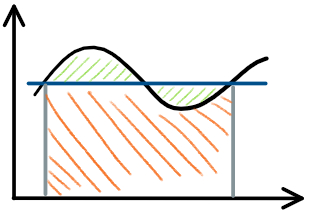
\includegraphics[scale=0.5]{Skizzen/mws_int}
	\end{center}
	\caption{Mittelwertsatz der Integralrechnung}
	\label{plot_MWS_int}
	\end{figure}		
	
	Dann existiert ein $\xi \in [a,b]$ mit 
	\begin{align*}
		\int_a^b f g \dd{x} = f(\xi) \int_a^b g\dd{x}
	\end{align*}
	\textbf{Bemerkung:}
	Für $g = 1$ gilt dann: 
	\begin{align*}
		\int_a^b f \dd{x} = f(\xi) \cdot (b-a)
	\end{align*}
}\end{Satz}

\begin{proof}
 	Man setze: $h: [a,b] \rightarrow \mathbb{R},$ $y \mapsto f(y) 
	\cdot \int_a^b g \dd{x}$. $h$ ist stetig und es gilt:
	\begin{align*}
		\inf_{y \in [a,b]} h(y) = & \inf_{y \in [a,b]} \int_a^b f(y) g(x) \dd{x} \\
		\leq & \int_a^b \int_{y \in [a,b]} f(y) g(x) \dd{x} \\
		 \overset{Satz~\ref{vl_11_satz24}}{\le} & \int_a^bf(x)g(x) \dd{x} 
		\overset{Satz~\ref{vl_11_satz24}}{\le}
		\int_a^b \sup_{y \in [a,b]} f(y) g(x) \dd{x} = \sup_{y \in [a,b]} h(y)
	\end{align*}
	Das heißt wir haben eine stetige Funktion $h$ mit: 
	\begin{align*}
		\int_a^b fg\dd{x} \in [\inf_{y \in [a,b]} h(y),  \sup_{y \in [a,b]} h(y)]
	\end{align*}
\end{proof}

\begin{Bemerkung}{
	 Wir haben bereits gesehen: Polynome sind beliebig oft
	 differenzierbar.	
}\end{Bemerkung}
